
\begin{figure}
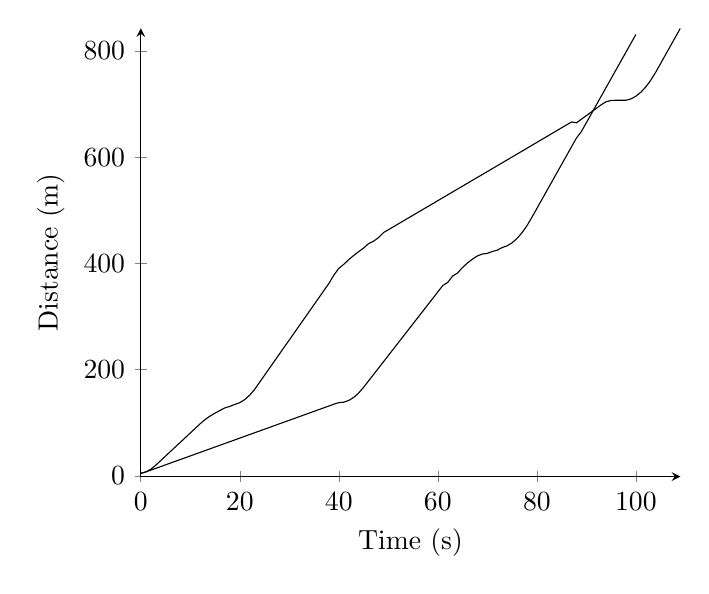
\begin{tikzpicture}
\begin{axis}[
legend style={anchor=west},
axis x line=bottom,
axis y line=left,
ymin=-1,
xlabel=Time (s),
ylabel=Distance (m),
]
\addplot[] coordinates {
(0, 5.1)
(1, 7.6)
(2, 10.9543761746)
(3, 14.3087600282)
(4, 17.6631521417)
(5, 21.0175531562)
(6, 24.3719637809)
(7, 27.7263848022)
(8, 31.0808170952)
(9, 34.4352616359)
(10, 37.7897195164)
(11, 41.1441919627)
(12, 44.498680356)
(13, 47.8531862581)
(14, 51.2077114416)
(15, 54.5622579271)
(16, 57.9168280282)
(17, 61.2714244064)
(18, 64.6260501395)
(19, 67.980708806)
(20, 71.3354045917)
(21, 74.6901424247)
(22, 78.0449281473)
(23, 81.3997687394)
(24, 84.7546726098)
(25, 88.1096499828)
(26, 91.4647134179)
(27, 94.8198785189)
(28, 98.1751649196)
(29, 101.530597682)
(30, 104.886209319)
(31, 108.242042811)
(32, 111.598156209)
(33, 114.954629953)
(34, 118.311578941)
(35, 121.669173485)
(36, 125.027678003)
(37, 128.387528325)
(38, 131.749503499)
(39, 135.115170515)
(40, 138.164919341)
(41, 138.895518713)
(42, 142.126118085)
(43, 147.856717457)
(44, 156.087316829)
(45, 166.817916201)
(46, 178.786798961)
(47, 190.755923303)
(48, 202.7253237)
(49, 214.695041511)
(50, 226.665126794)
(51, 238.635640715)
(52, 250.606658814)
(53, 262.578275488)
(54, 274.55061027)
(55, 286.52381679)
(56, 298.498095867)
(57, 310.473715137)
(58, 322.451039364)
(59, 334.430578901)
(60, 346.413070385)
(61, 358.399617796)
(62, 364.261954092)
(63, 376.26520703)
(64, 382.043258866)
(65, 392.434704567)
(66, 400.916465309)
(67, 408.10985629)
(68, 414.127579265)
(69, 417.711240636)
(70, 418.885608861)
(71, 422.420044334)
(72, 424.883380285)
(73, 429.846716237)
(74, 433.066228434)
(75, 438.785740632)
(76, 447.005252829)
(77, 457.724765027)
(78, 470.944277225)
(79, 486.663789422)
(80, 503.263789422)
(81, 519.863789422)
(82, 536.463789422)
(83, 553.063789422)
(84, 569.563789422)
(85, 586.163789422)
(86, 602.763789422)
(87, 619.363789422)
(88, 635.963789422)
(89, 648.103789422)
(90, 664.703789422)
(91, 681.303789422)
(92, 697.903789422)
(93, 714.503789422)
(94, 731.103789422)
(95, 747.703789422)
(96, 764.303789422)
(97, 780.903789422)
(98, 797.503789422)
(99, 814.103789422)
(100, 830.703789422)
};
\addplot[] coordinates {
(0, 5.1)
(1, 7.6)
(2, 12.6)
(3, 20.1)
(4, 28.7907787796)
(5, 37.4816321233)
(6, 46.1725783063)
(7, 54.8636421116)
(8, 63.5548580118)
(9, 72.2462754229)
(10, 80.9379677972)
(11, 89.6300492856)
(12, 98.3227075284)
(13, 106.323306923)
(14, 112.796690249)
(15, 118.351101101)
(16, 123.41883034)
(17, 128.235572524)
(18, 131.067286152)
(19, 134.701431802)
(20, 138.021454247)
(21, 143.841476692)
(22, 152.161499137)
(23, 162.981521583)
(24, 176.301544028)
(25, 189.591720436)
(26, 202.877734512)
(27, 216.163891784)
(28, 229.450217586)
(29, 242.736743597)
(30, 256.023509972)
(31, 269.310568367)
(32, 282.597986386)
(33, 295.885854239)
(34, 309.174295061)
(35, 322.463481433)
(36, 335.753662971)
(37, 349.045214698)
(38, 362.338727085)
(39, 377.897001157)
(40, 390.677141451)
(41, 398.229995089)
(42, 407.132396434)
(43, 414.919231282)
(44, 422.02306896)
(45, 428.768997418)
(46, 437.22762913)
(47, 441.598186031)
(48, 448.468742932)
(49, 457.839299833)
(50, 463.312917435)
(51, 468.786706132)
(52, 474.260677398)
(53, 479.734843759)
(54, 485.209218911)
(55, 490.683817865)
(56, 496.158657108)
(57, 501.633754786)
(58, 507.109130923)
(59, 512.584807665)
(60, 518.060809576)
(61, 523.53716397)
(62, 529.013901313)
(63, 534.491055688)
(64, 539.96866535)
(65, 545.446773387)
(66, 550.925428506)
(67, 556.404685983)
(68, 561.884608807)
(69, 567.265269084)
(70, 572.754837064)
(71, 578.244502847)
(72, 583.734278326)
(73, 589.224177411)
(74, 594.71421647)
(75, 600.204414903)
(76, 605.694795875)
(77, 611.18538728)
(78, 616.67622302)
(79, 622.167344716)
(80, 627.658804045)
(81, 633.150665991)
(82, 638.643013438)
(83, 644.135953833)
(84, 649.62962907)
(85, 655.124230621)
(86, 660.619845636)
(87, 666.11616605)
(88, 664.539524442)
(89, 671.272526528)
(90, 678.018182)
(91, 684.78416796)
(92, 691.586303669)
(93, 698.464471497)
(94, 704.224843176)
(95, 706.542407837)
(96, 706.974445302)
(97, 706.98997989)
(98, 706.98997989)
(99, 709.48997989)
(100, 714.48997989)
(101, 721.98997989)
(102, 731.98997989)
(103, 744.48997989)
(104, 759.48997989)
(105, 776.08997989)
(106, 792.68997989)
(107, 809.28997989)
(108, 825.88997989)
(109, 842.48997989)
};

\end{axis}
\end{tikzpicture}
\label{tik:distance:100:71}
\caption{100 percent diving with GSC on route $71$}
\end{figure}
